\section{The eBPF Programmer Gap}
\label{sec:motivation}

While eBPF verification is important for program safety, the eBPF verifier
    places additional constraints on programs, which results in usability challenges.
The core of the problem is a large gap between the programmer and the
    verifier.
Typical eBPF development involves implementing programs in a high-level
    programming language (e.g., C, Rust) and compiling to eBPF bytecode.
Developers agree to a contract with the high-level language, which is
    enforced by the compiler.
When a program fails to compile, the developer will get a message with
    hints about where they violated
    the contract with the programming language.
If, however, a program fails to pass the verifier it is harder for the programmer
    to understand why the program failed and how to fix it.
\mvle{not clear why it is hard for the programmer to understand verification failure messages.
Is it because what is being verified is not the same program being written and not the
same semantics being checked at the higher-level language?}
In order to quantify the impact of this gap,
    we analyzed commit messages from popular eBPF projects to see how programmers fix
    eBPF programs that fail to verify.
From the commit messages, we created a set of categories of fixes.
In the rest of this section we will describe our methodology and categorization, walk through some illustrative examples, and describe the key high level takeaways which are that the programmer gap as described exists, and that it makes the eBPF system less usable.
\milo{Reword this last sentence}

%Additionally, we describe two fundamental reasons for the programmer gap.
\milo{succinctly say them here.}



%At the same time, the verifier has a set of properties that it ensures are maintained for each program, such as memory safety.
%The verifier will reject programs that do not meet these properties.
%The compiler does not know the set of properties that the eBPF verifier checks, which
%    introduces a gap between the compiler and the verifier, and, by extension, the programmer and the verifier.
%
%The problem is compounded by the fact that the verifier operates on code that has undergone
%    translation from a high-level language into eBPF bytecode.
%The cause of verifier rejections may unrelated to the code the programmer wrote and instead
%    be a result of bugs anywhere along the toolchain.
%The verifier is also a moving target, with different versions having different constraints
%    and different completeness guarantees.
%As a result, eBPF developers often have to wrestle with the in-kernel verifier
%    to allow safe programs they write to pass.
%This can manifest itself in needing to write arcane expressions to please the
%    verifier, or by completely restructuring semantically correct and safe code.

%The compiler does not know the set of properties that the eBPF verifier checks, which makes it more difficult for developers to know if their program will run until they run the verifier.

%This binds developers with a contract not only with the high-level language
%    that is enforced by the compiler or interpreter, but also with the eBPF
%    verifier, where the specifications are not clear. \mvle{I don't it's an issue with specification. it's partly due to going from a turing-complete language to turing-incomplete. I think we should bulletize these challenges. 1. semantic gap (turing complete -> turing-incomplete, 2. difficult to debug due to many levels of translation, 3. compiler optimizations that are incompatible with verifier, 4. specification for verifier changes across kernel versions, 5. ?}
%Developers have a contract with the programming language that is enforced by the compiler of interpreter.
%The programmer also has a contract with the eBPF verifier, but the specifics are unclear.
%At the same time, because source code goes through a translation to eBPF
%    bytecode before verification, it is often difficult to map the verifier
%    error back to source code.
%Source code goes through a translation to eBPF bytecode before it is verified, which makes mapping the output of the verifier back to the code the programmer wrote difficult.

%To better understand this gap and the kinds of usability issues eBPF
%    developers face, we carried out an analysis on existing eBPF projects and
%    past research literature.
%We carried out an analysis of existing eBPF projects and research papers to better understand this gap and the kinds of verifier issues the eBPF developers face.
% eBPF developers often have to wrestle with the in-kernel verifier to allow the programs they write to pass.
% This can manifest itself in needing to write arcane expressions to please the verifier.
%We categorize the solutions that programmers need to implement in order to pass the verifier to get a clearer picture of the usability challenges that the current eBPF system has.

\subsection{Methodology}
To collect data, we searched through the git commit logs of Cilium, Aya-rs, and
    Katran \mvle{(need references for each project)}, which are mature, widely-used eBPF projects, for instances of
    keywords: "error", "reject", "rejects", "issue", and "verifier."
For each commit log that matched, we manually inspected and classified the commit.
In total, we collected 216 commit messages containing the above keywords, of which we decided that 73 of them were actually about verifier complaints.
In addition, we included two issues raised in the BMC~\cite{BMC} and Electrode~\cite{Electrode} papers as examples when appropriate.

%88\% of commit messages found were from the Cilium repository.
%Cilium is a mature project that makes extensive use of eBPF as a core part of its architecture.
%Cilium represents a representative set of challenges for large projects with complex eBPF code bases.
%\jinghao{Is this paragraph necessary?}

To classify the commits into categories, we read each of the commit messages and examined
    their source code changes.
Some categories were clear to see and are well documented in the literature (i.e. restructuring eBPF programs), while other categories were more subtle.
%We created a qualitative analysis of many of the kinds of fixes that are used when writing and verifying eBPF programs.

%The categorizations that we created are not necessarily mutually exclusive.
%We started with a large set of smaller categories, and then combined categories to
%    create larger categories that represented classes of fixes, as well as picking out
%    common patterns that are representative.

\subsection{Categorization Overview}

\begin{table}[t]
    \small
    \centering
    \begin{tabular}{lc}%{|p{6cm}|p{1cm}|}
        \toprule
        \textbf{Category} & \textbf{Count} \\
        \midrule
        Change source code to fix LLVM codegen & 22 \\          % #1
        Restructure eBPF program for verifier & 20 \\           % #2
        Add specific code to pass verifier & 17 \\              % #3
        Implement kernel-version-specific fixes & 9 \\          % #4
        Add "pruning checkpoints" to reduce complexity & 7 \\   % #5
        % moved to #2 Refactor code because of lack of expressiveness & 2 \\
        % moved to #2 Split eBPF programs for complexity & 13 \\
        % moved to #2 Refactor code to reduce complexity & 5 \\
        % moved to #3 Inline functions to pass verifier & 6 \\
        % moved to #3 Explicitly teach the verifier information & 6 \\
        % moved to #3 Add bounds to a helping function & 3 \\
        % moved to #3 Add a specific implementation of a helping function & 2 \\
        \bottomrule
    \end{tabular}
    \caption{Table of common verifier problems. \mvle{we should rename these categories. These don't sound like verifier problems but actions done to overcome verfier issues.}}
    \label{fig:commit-table}
\end{table}

Our analysis classifies the commits into five categories.
Each category represents a class of techniques that developers used to make their programs pass the verifier.
Table~\ref{fig:commit-table} summarizes the results of our analysis.

%\jinghao{
%Some comments on the table: it is not immediately clear on what exactly
%    the developers are doing for some of the categories, especially the last
%    3. (btw, should it be ``helper functions'' or ``helping functions'').
%At the same time, the categories do not seem to be mutually exclusive,
%    e.g., ``Split eBPF programs for complexity'' vs.
%    ``Refactor code to reduce complexity''.
%We should be clear whether the categories are overlapping.
%}

The composition of the categories makes it clear that developers have to change their code in particular ways to get it to pass the verifier.
It also demonstrates how difficult it can be to reason about the results of the verifier.

There are two basic reasons an eBPF program can fail to verify. %for several reasons.
The first reason is when the program is unsafe, and the verifier correctly rejects it.
The second reason is when a program is actually safe but the verifier is overly conservative
in how it checks the program, and thus rejects it.
When the verifier rejects a safe program, it is up to the developer to find a way to show the verifier that the program actually is safe.
The classes of solution employed are different ways that developers use to make sure the verifier accepts their programs.
%\jinghao{This paragraph is reptitative given the preamable, I think what is
%    missing here is an overview of the finding from our study (i.e. beef up the
%    previous paragraph)}

\subsection{Category Representative Examples}
To better explain our categorization, we now walk through some representative examples for the most important categories.

\subsubsection{Change Source Code to Fix LLVM Codegen}
\label{motivation:llvm-codegen}
The LLVM compiler translates eBPF programs written in high-level languages into eBPF bytecode.
We found that in certain cases, LLVM would generate eBPF bytecode that would cause the program to fail verification.
One issue found by Cilium was that LLVM may generate 32-bit assignments for
    accessing \texttt{ctx->data}, \texttt{ctx->data\_end}, \texttt{ctx->data\_meta} fields as
    each of the fields are on 32-bit boundaries.
However, the verifier cannot track the packet pointers through these 32-bit assignments and
    will cause the program to fail to verify.
As shown in Figure~\ref{fig:inline-error}, R9 is a pointer to a packet in instruction 2.
At instruction 3, R6 gets the value of R9, but this is a 32-bit assignment, as indicated by the `w' prefix.
Then in the next line we see that R6 has type `inv' which is a scalar value, and \emph{not} a pointer to a packet showing that the verifier lost track of the type of R6.

%The \texttt{data} field is
The LLVM compiler thought that the \texttt{data} fields were 32-bit values as 
    a result of the information hiding techique that
    eBPF employs.
The kernel exports a context interface to the extension program with only
    the fields that program may need, and at verification time all accesses to
    these fields are rewritten by the verifier to the actual kernel-internal
    data structure.
Since the \texttt{data} field is defined as a 32-bit integer in the dummy
    interface the kernel exports, the compiler, which does not see the
    subsequent rewriting and kernel-internal definition, treats it as a real
    32-bit integer and performs code generation, even though \texttt{data} is
    supposely a 64-bit pointer.

The solution was to implement the access through inline assembly code shown in Figure~\ref{fig:inline-asm}.
This prevents LLVM from generating 32-bit assignments as an optimization because it must leave the assembly as it is.
This then allows the verifier to track that the register still contains a packet pointer, and not a scalar value.
%\jinghao{It is actually not too clear how this fixes the problem -- for
%specifically how is the generated code different?}
%\jinghao{can we be more specific on the BPF opcode (e.g., load/store) of the
%    assignment as in Figure~\ref{fig:inline-asm}}


This workaround allows the eBPF program to pass the verifier.
It is clear that this exposes usability issues of the verifier.
The LLVM compiler is unaware of the verifier's needs, and the programmer must know low level detail about the eBPF system and LLVM bytecode generation in order to realize this.

Another change that was implemented was to mark certain variables as \texttt{volatile}
to keep LLVM from performing other kinds of optimizations that would cause the program to be rejected by the verifier.

\begin{figure}
    \lstinputlisting[language=myBPF]{./snippets/s2-codegen-error.c}
    \caption{Verifier log for LLVM generated 32-bit assignment}
    \label{fig:inline-error}
\end{figure}

\begin{figure}
    \lstinputlisting[language=myC]{./snippets/s2-inline-asm.c}
    \caption{Inline asm to access fields}
    \label{fig:inline-asm}
\end{figure}


\subsubsection{Restructure eBPF program for verifier}
\label{motivation:restructure}
A big theme across the commits we found was the need to explicitly restructure eBPF programs to pass the verifier.
We identified two main techniques for restructuring programs:

\begin{enumerate}
    \item Split eBPF programs into smaller subprograms
    \item General refactoring to reduce verifier complexity or bypass expressiveness limits
\end{enumerate}

\noindent\textbf{Splitting eBPF Programs}:
A well documented technique to decrease overall eBPF program complexity is to use eBPF tail calls to split programs into several smaller subprograms that can be verified independently.
The idea behind the split is that if each individual piece is verified to be safe, then the verifier itself would have verified the entire program if it could check enough instructions.
Prior works like BPF Memcahced Cache (BMC)~\cite{BMC} and Electrode~\cite{Electrode} utilize this technique in order to pass the verifier.
BMC is split into seven different eBPF programs, and Electrode is split into six different eBPF programs.
Both of these projects use around 500 lines of C code to program the eBPF programs.

Modularity is good when programmers can split their code up into logical units, however due to the constraints of the verifier, they must split their code to match the verifier.
In this case, we are left with program fragments which do not represent an individual unit, which makes the code harder to read and write.
This compounds with the fact that the compiler has no notion of these limits.
The compiler would happily compile both the split versions of code and the unified version of code, however only one set of code would pass the verifier.
Additionally, it is not necessarily trivial to split these functions because all safety checks need to be made in each subfunction in order for them to be independently verified.
We will now explore BMC as a representative example of this class of fix.
%\jinghao{Why is this the case?
%I think there are 2 cases, one is that the developers can just
%split the program at the logical boundaries so that they actually get the
%modularity; the other case is that they simply cannot split the program at these
%boundaries and have to break it into fragments, I think this is what we are
%arguing for and we have already seen in the case of BMC where they have to
%keep a ``parse context'' across tail calls.}

BMC~\cite{BMC} is an in-kernel cache for Memcached
    based on eBPF.
BMC stores recently queried key-value pairs in an eBPF map (i.e. the cache) to
    accelerate the processing of GET requests to the Memcached server.
If a GET is hit in the cache, BMC can directly draft a reply to send back the
    queried value without going through the expensive Linux network stack.
% The map that serves as the cache is managed by eBPF programs, which implements
%     the lookup and update logics.impl:ctx-converison

Implementation-wise, BMC is much more complicated
    comparing to other common eBPF use cases.
In order to pass the verifier, it has to be split into seven
    eBPF programs that use eBPF tail calls to transfer control to each other to
    reduce verification complexity.
Similar problem also presents when processing the incoming packet data, where
    the authors had to bound data size to simplify verification of loops.

%In the initial design of \projname{}-BMC, the underlying assumption was that
%    we should follow the logic of BMC.
%But the cache invalidation function Figure~\ref{fig:bmc-code} in BMC employs
%    \texttt{for} loops with cumbersome condition checks, and is further
%    complicated by the nesting of multiple \texttt{if} statements.

A representative example where BMC suffers from the verifier is its cache
    invalidation function, shown in Figure~\ref{fig:bmc-code}.
The cache invalidation code employs \texttt{for} loops with cumbersome
    condition checks, and is further complicated by the nesting of multiple
    \texttt{if} statements.

The complexity is exacerbated by introducing two additional variables to track
    the state of the key and the SET command.
% \jinghao{Let me know if removing this makes sense: ``and the end of packet''.}
Such complex checks are intentionally designed to pass the
    verifier.
Without these checks, the program produces an excessive number of jump instructions,
    leading to verification failure.
% the verifier to reject loading the program.
This approach significantly increase the programming burden
    of BMC, while at the same time leads to readability issues in some places
    regarding the intended functionality.
% \jinghao{One or two sentence explain why conditions are needed for
%     verification, based on our experiment on removing one of these.}
% This situations is a prevalent pattern within the BMC structure, which is
Such pattern is prevalent in the BMC implementation, which is
%    notably observed within the functions \texttt{bmc\_hash\_keys\_main}
%    and \texttt{bmc\_write\_reply\_main}.
    notably also present in the code that hashes the Memcached key and drafts the reply.

Another example that the verifier creates programming burden for BMC is its
    instruction count limit.
% Due to the instruction count limitation imposed on each eBPF program,
%     BMC has to adapt a strategy of creating seven seperated eBPF
%     programs to function as a Memcached cache layer.
Due this limit, BMC has to be split into seven seperated eBPF program, while
    ideally only two are required (at egress and ingress hooks).
Unfortunately, this leaves program fragments that are not self-contained and
    BMC sometimes has to pass computation states across tail calls.
% To pass messages across tail calls, BMC employed a specific struct
%     called \texttt{parsing\_context} for storing the metadata and
%     put the struct in the map named \texttt{map\_parsing\_context}.
BMC utilizes a map to pass current computation state across tail calls.
This is because tail-called eBPF programs can only take the regular eBPF
    context as arguments.
The computation state is stored before the tail call and reloaded afterwards.

\jinghao{Currently just dumping text -- needs to incorporate BMC here somehow}

% The BMC has many places where for loops are nested into different ifs.
% And, due to the limitations of C, many operations do not have built-in functions
%     that can be used directly.

\begin{figure}[t]
    \lstinputlisting[language=myC]{./snippets/s6-bmc.c}
    \caption{Packet parsing code for cache invalidation in BMC}
    \label{fig:bmc-code}
\end{figure}

\noindent\textbf{Refactoring Code}:
Code may also need to be refactored to reduce its complexity, or to work around limitations in the verifier.
One example of refactoring for complexity found in a Cilium commit involved changing how the code handled IPv4 fragmentation.
As seen in Figure~\ref{fig:refactor-fix} the code used an \texttt{\#ifdef} with a default behavior.
If \texttt{ENABLE\_IPV4\_FRAGMENTS} was enabled, then the code would be compiled with both the \texttt{ipv4\_handle\_fragment} call and the \texttt{ctx\_load\_bytes} call.
%If the packet was a fragment, then the \texttt{ipv4\_handle\_fragment} call would have completed the loading of bytes, and the additional call would have been redundent.
%\jinghao{I recommend removing this last sentence. It makes it sounds like a
%good thing that developers have to remove some redundent code.}

This design however, caused the program to fail verification as it went over the maximum checked instruction limit.
The code was then refactored to change the \texttt{\#ifdef} and the underlying function.
This change does not change the safety properties of the program, but it was still needed to verify the program.

\begin{figure}
    \lstinputlisting[language=myC]{./snippets/s2-refactor.c}
    \caption{Refactor for Code Complexity}
    \label{fig:refactor-fix}
\end{figure}


We found an example of refactoring for expressiveness in the Cilium project.
To implement segment routing header support, they needed to include code to jump to IP header parsing code while already inside the IP header parsing code.
This would cause a back-edge which gets incorrectly labeled as an infinite loop and the verifier fails.
Figure~\ref{fig:switch} shows their solution which involved creating a switch statement inside of a switch statement which then jumps ahead to the other code in the outer switch statement.
The changes required increase the complexity of the source code without changing the semantics.

\begin{figure}
    \lstinputlisting[language=myC]{./snippets/s2-switch.c}
    \caption{Refactor for Expressiveness}
    \label{fig:switch}
\end{figure}

\subsubsection{Add specific code to pass verifier}
\label{motivation:add-code}
Another common fix for verifier complaints involves adding specific code to please
    the verifier.
This can involve several kinds of new specific code:

\begin{enumerate}
    \item Adding inline functions
    \item Teaching the verifier information
    \item Implementing functions in a specific way
\end{enumerate}

\noindent\textbf{Inlining Functions to Pass Verifier}:
The verifier can lose track of information depending on how eBPF programs are structured.
One fix for this is to inline functions for implementing functionality.
It is not always clear what code needs to be made into a inlined function for the verifier
    which makes eBPF less usable.

\begin{figure}
    \lstinputlisting[language=myC]{./snippets/s2-goto.c}
    \caption{Goto transformed to inline function}
    \label{fig:inline-fig}
\end{figure}

%\begin{figure}
%    \begin{lstlisting}[language=myC]
%policy_check_entry:
%	account(ctx, policy);
%
%	if (unlikely(policy->deny))
%		return DROP_POLICY_DENY;
%
%	*proxy_port = policy->proxy_port;
%	if (unlikely(policy->auth_type)) {
%		if (ext_err)
%			*ext_err = (__s8)policy->auth_type;
%		return DROP_POLICY_AUTH_REQUIRED;
%	}
%	return CTX_ACT_OK;
%}
%    \end{lstlisting}
%    \caption{Block of code reached after a goto}
%    \label{fig:inline-fig}
%\end{figure}

We found an example of this in Cilium.
Code that performed policy checks used goto statements to prevent code duplication.
As seen in Figure~\ref{fig:inline-fig} the \texttt{policy} variable could be used to refer to \texttt{policy} or \texttt{l4policy} before jumping to the checking logic.
This caused the verifier to reject the program because it lost track of what the \texttt{policy} variable referred to.
The developers fixed this by converting the policy check logic from a labeled block of code, to an inline function.
The original structure of the code before was valid and correct, but it failed to pass the verifier.
In response to this, the developers had to figure out a workaround to make their valid code pass.

%The developers made this code general across two cases by reassigning the value of policy depending on what the input was before jumping to the common code.
%This pattern caused the verifier to lose information about what the variable \{policy{ was referring to.
%The fix was to convert this common code into an inlined function.
%\jinghao{
%It is hard to see why this is a problem, especially when you say ``Doing this
%    helps to keep functionality separate from the programmers perspective,
%    while allowing the verifier to see all the code at the same time''.
%I think we need something similar to the previous cases where we explicitly
%    discuss why it is bad.
%}

\noindent\textbf{Explicitly teaching the verifier information}
%An example of explicitly teaching the verifier information can be found in the Aya-rs project.
%As part of their library, Aya contains functions to help log information.
%Throughout the project they have an upper bound on the size of the log buffer.
%In a write string function they needed to add an explicit check on the size of the length of the string against the log buffer max size.
We found an example in Cilium where the developer needed to explicitly teach the verifier
    information.
The verifier lost track of the value of \texttt{nh\_params.nh\_family}, which caused it to reject the program.
In Figure~\ref{fig:teach-verifier}, we can see that the developers needed to slightly change the code in order to ensure the verifier knew what the value was.
The original code was fully safe, but the verifier rejected it.
The required fix is also counter-intuitive, which makes it less usable.

\begin{figure}
    \lstinputlisting[language=myC]{./snippets/s2-teach.c}
    \caption{Teaching the verifier info}
    \label{fig:teach-verifier}
\end{figure}

\noindent\textbf{Implementing functions in a specific way}
We found examples of this in both Cilium and Aya-rs.
Both of these projects found uses for the functions \texttt{memset} and \texttt{memcpy}, but they had to provide their own versions of them.
Aya-rs took the approach of writing a simple version shown in Figure~\ref{fig:aya-memcpy}, while Cilium uses a much more complicated approach, a portion of which is shown in Figure~\ref{fig:cilium-memcpy}.
Both of these code snippets were designed to pass the verifier.
\milo{The cilium one was not found in a commit but should I add it to the counts?}

\begin{figure}
    \begin{lstlisting}[language=rust]
#[no_mangle]
pub unsafe extern "C" fn memcpy(dest: *mut u8, src: *mut u8, n: usize) {
    let dest_base = dest as usize;
    let src_base = src as usize;
    for i in 0..n {
        *((dest_base + i) as *mut u8) = *((src_base + i) as *mut u8);
    }
}
    \end{lstlisting}
    \caption{Simple and specific implementation of memcpy}
    \label{fig:aya-memcpy}
\end{figure}

\begin{figure}
    \lstinputlisting[language=myC]{./snippets/s2-cilium-memcpy.c}
    \caption{Memcpy implementation in Cilium}
    \label{fig:cilium-memcpy}
\end{figure}

\subsubsection{Implement kernel-version-specific fixes}
\label{motivation:kernel-version}
Different kernel versions may have different versions of the eBPF verifier, each with different sets of bugs.
To maintain compatibility between these versions, developers have to change code to account for the differences.
A good example of this is found in Cilium.
The verifier failed the program with the message shown in Figure~\ref{fig:kernel-version}.
This is a known verifier bug that has been fixed, but the fix is not present in all kernel versions.
Cilium developers had to implement a simple, but precise fix to ensure that the program would verify on all extensions.
As shown in Figure~\ref{fig:kernel-version-code} the fix needed was to move line 7 to line 1 before the block of code.

\begin{figure}
    \begin{lstlisting}[language=myBPF]
1411: (bf) r1 = r9
1412: (07) r1 += 48
1413: (67) r2 <<= 16
1414: (47) r2 |= 512
1415: (63) *(u32 *)(r1 +0) = r2
; dereference of modified ctx ptr R1 off=48+0,
; ctx+const is allowed, ctx+const+const is not
    \end{lstlisting}
    \caption{Verifier output showing error}
    \label{fig:kernel-version}
\end{figure}

\begin{figure}
    \lstinputlisting[language=myC]{./snippets/s2-kernel-version.c}
    \caption{Kernel version specific fix}
    \label{fig:kernel-version-code}
\end{figure}

\subsubsection{Add Pruning Checkpoints}
\label{motivation:checkpoint}
Another common fix that Cilium implemented was to introduce a pseudo-helper function \texttt{relax\_verifier}.
The purpose of this helper is to provide a checkpoint for the verifier to use when doing state pruning.
All the function does it call a kernel helper function, which then introduces a new state pruning checkpoint.
%\jinghao{Can we put more information here on this helper? It would be great
%to show that the helper itself is complicated and developers have to insert it
%at random places.}
%\jinghao{My understanding is that this calls a \textit{kernel helper} so that the
%state is reset?}
In some cases doing so significantly decreases the complexity of eBPF programs.
In one commit, doing so reduced the number of instructions checked from 62,569 to 49,669.
This is more significant on older kernel versions which have a much smaller upper limit to the number of instructions the eBPF verifier could check.
\jinghao{It now seems to me that this belongs to \S~\ref{motivation:restructure}.}
\milo{I don't think so because the state pruning knowledge is more obscure, so needing to use it is harder than refactoring. i.e. A dev may know that their loops can't be too complicated, but they may not know anything about verifier internal state pruning? It also does not really change the structure (this is intentional)}

With no assistance, programmers are required to have knowledge of low-level
    internal details of the eBPF verifier, and then implement fixes that
    make use of this knowledge.
Having to make this change harms the usability of eBPF.


\subsection{Analysis Takeaways}
From our analysis, we believe that there are serious usability challenges to the
    existing eBPF system that stem from the gap between programmer and verifier.
The categories of verifier issue that we found are direct indicators of this problem.
eBPF programmers have to implement arcane fixes and change their mental model of
    programming to meet the constraints of the verifier without any assistance.
If an eBPF program fails to verify there is not always a clear reason why that was the case, e.g.,
it could be that a programmer's source code was completely safe, but LLVM generated code that the verifier did not understand.
To programmers, a successful compilation should indicate something about the success of their code, but in the eBPF system that is not the case.
This gap is fundamental to the eBPF system.
A system that closes this gap by moving the verifier and the compiler closer together may be able to avoid the challenges discovered in the existing eBPF system, while still maintaing many of the safety properties.
% \jinghao{would be interesting to talk about saving/reloading computation
%     context across tail calls}

%Different kernel versions have different verifiers with different constraints
%    and different properties that they check.
%There would have to be some way to fully expose the specifics of the verifier
%    back to the compiler to close the gap.

%\subsection{Mismatches Cause the Gap}
%In this section we examine two of the main causes of the programmer gap.
%The programmer gap is a consequence of two mismatches between the verifier and the compiler that arises due to the design of the eBPF system.
%    \begin{enumerate}
%        \item Version mismatches
%        \item Safety mismatches
%    \end{enumerate}

%\subsubsection{Version Mismatches}
%There are three sources of versioning that eBPF currently has, that may lead to issues.
%\begin{enumerate}
%    \item Kernel Interface
%    \item Verifier
%    \item Compiler
%\end{enumerate}
%
%Kernel interface version problems are resolved by the use of BTF and CO-RE in BPF.
%However, the version issues differences between the compiler and verifier are not dealt
%    with in any way.
%
%In the current eBPF system, the compiler and the verifier are decoupled.
%As development proceeds, implementation details about the compiler and verifier change.
%As seen in Table~\ref{fig:commit-table} there are examples of differences in implementation
%    between the LLVM compiler toolchain and the eBPF verifier breaking
%    program verification.
%Figure~\ref{fig:2comp1ver} shows a flowchart of how this might happen.
%
%Problems can also arise from different verifier versions.
%If an eBPF program verifies on one version, there is no guarantee that it verifies on a different version.
%Examples of this include backwards compatibility for features like loops.
%Figure~\ref{fig:1comp2ver} shows a flowchart of how this might happen.
%
%There is no way to fully resolve the issues of versioning in the eBPF system as
%    each component is a constantly moving target.
%Compilers will continue to evolve, just as the eBPF verifier will continue to evolve, and because they are decoupled, there will be places where they do not align.

%\begin{figure}
%    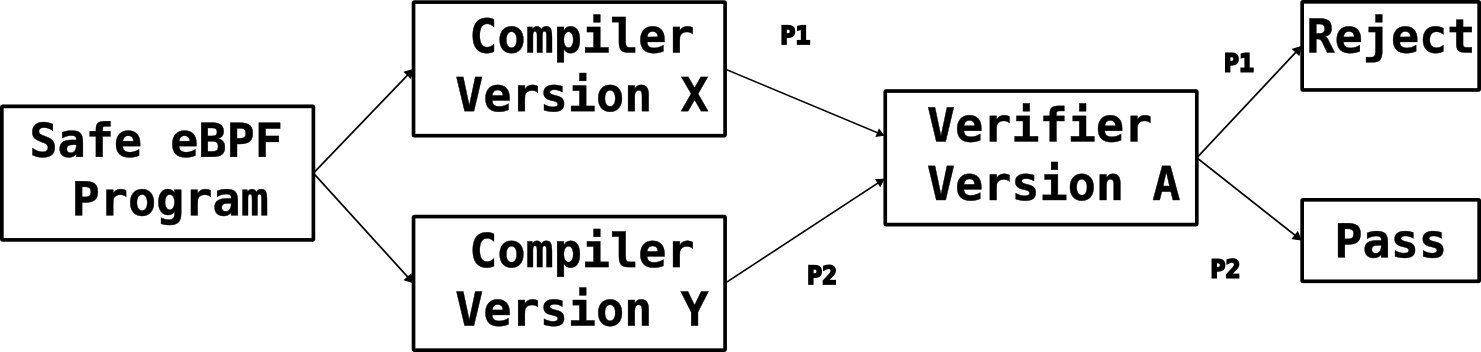
\includegraphics[width=1.0\linewidth]{figs/2comp1verifier}
%    \centering
%    \caption{Version issue between two compiler versions}
%    \label{fig:2comp1ver}
%\end{figure}
%
%\begin{figure}
%    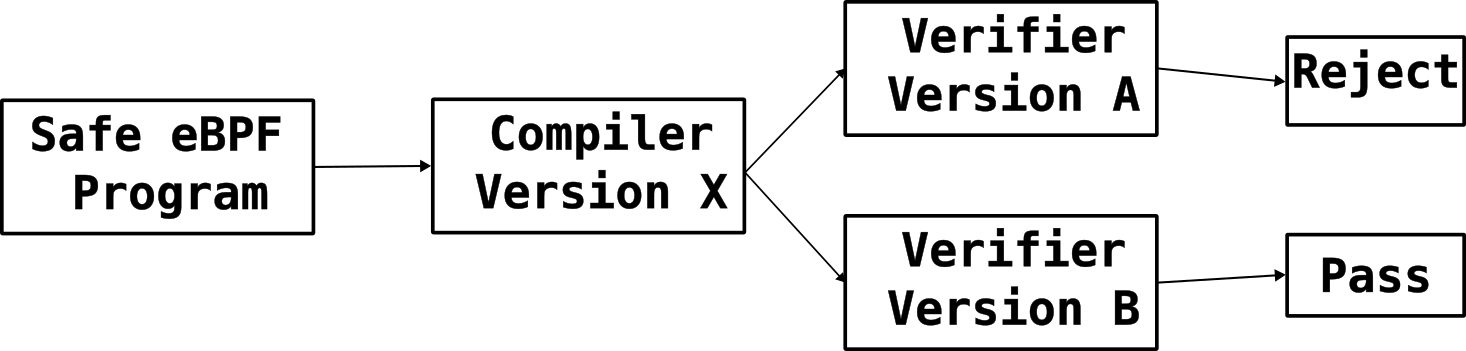
\includegraphics[width=1.0\linewidth]{figs/1comp2verifier}
%    \centering
%    \caption{Version issue between two verifier versions}
%    \label{fig:1comp2ver}
%\end{figure}




